% !TEX program = xelatex
% Proposal Project 1 -- converted from "Proposal Project1.docx"
% Compile with: xelatex main.tex (run twice for references/labels)
%
% File layout (edit content in sections/, not here):
%   sections/00-cover.tex        หน้าปก
%   sections/00-proposal-id.tex  หน้าเสนอเค้าโครงโครงงาน
%   sections/01-title.tex        1. ชื่อหัวข้อโครงงาน
%   sections/02-rationale.tex    2. หลักการและเหตุผล
%   sections/03-objectives.tex   3. วัตถุประสงค์ของโครงงาน
%   sections/04-theory.tex       4. ทฤษฎีและผลงานวิจัยที่เกี่ยวข้อง
%   sections/05-methodology.tex  5. วิธีดำเนินการวิจัย
%   sections/06-scope.tex        6. ขอบเขตและข้อจำกัดของการวิจัย
%   sections/07-location.tex     7. สถานที่ทำวิจัย
%   sections/08-benefits.tex     8. ประโยชน์ที่คาดว่าจะได้รับ
%   sections/09-timeline.tex     9. แผนและระยะเวลาดำเนินการ
%   sections/10-budget.tex       10. งบประมาณ
%   sections/11-references.tex   11. เอกสารอ้างอิง
%   sections/99-signature.tex    แบบฟอร์มรับรองจากที่ปรึกษา
\documentclass[a4paper]{article}

\usepackage{geometry}
\geometry{a4paper, top=1.5in, left=1.5in, right=1in, bottom=1in, headheight=1in}

\usepackage{fontspec}
\setmainfont{THSarabunNew.ttf}[
  Path = fonts/,
  BoldFont = {THSarabunNew Bold.ttf},
  ItalicFont = {THSarabunNew Italic.ttf},
  BoldItalicFont = {THSarabunNew BoldItalic.ttf}
]

\usepackage{graphicx}
\usepackage{xcolor}
\usepackage{colortbl}
\usepackage{array}
\usepackage{enumitem}
\usepackage{caption}
\usepackage[hidelinks]{hyperref}
\usepackage{titlesec}
\usepackage{setspace}
\usepackage{indentfirst} % indent the first paragraph after a heading too

% --- Thai figure/table caption names ---
\renewcommand{\figurename}{ภาพที่}
\renewcommand{\tablename}{ตารางที่}
\captionsetup{labelsep=quad, justification=centering, font=bf}

% --- Body content: headings "N.    หัวข้อ" size 14 bold (section) / size 14
% normal (subsection, subsubsection), body text size 14 normal.
%
% Cascading indent: each level's number starts where the PREVIOUS level's
% title text started, so the outline steps inward one level at a time
% instead of every level sharing one column:
%   5.      วิธีดำเนินการวิจัย            <- number at 0,      title at \lvlA
%           5.1   การศึกษา...             <- number at \lvlA,  title at \lvlB
%                 5.1.1   การศึกษา...     <- number at \lvlB,  title at \lvlC
% The section-number box leaves a ~4-space gap after the number; the
% subsection/subsubsection boxes leave a ~2-space gap (per spec). Body
% paragraphs under each level are indented (via \global\parindent, set in
% each heading's "before" hook) to line up with that level's title text.
% Widths are measured (not guessed) so the gap is exactly 4 real interword
% spaces after a section number, and exactly 2 after a subsection/subsubsection
% number -- "11." is the widest section number in this document, "4.1" /
% "4.2.1" are representative since every subsection/subsubsection number in
% this document is the same character length at its level.
\newlength{\lvlOneBox}
\newlength{\lvlTwoBox}
\newlength{\lvlThreeBox}
\newlength{\fourspace}
\newlength{\twospace}
\settowidth{\fourspace}{\fontsize{14}{17}\selectfont\bfseries\ \ \ \ }
\settowidth{\twospace}{\fontsize{14}{17}\selectfont\normalfont\ \ }
\settowidth{\lvlOneBox}{\fontsize{14}{17}\selectfont\bfseries 11.}
\addtolength{\lvlOneBox}{\fourspace}
\settowidth{\lvlTwoBox}{\fontsize{14}{17}\selectfont\normalfont 4.1}
\addtolength{\lvlTwoBox}{\twospace}
\settowidth{\lvlThreeBox}{\fontsize{14}{17}\selectfont\normalfont 4.2.1}
\addtolength{\lvlThreeBox}{\twospace}

\newlength{\lvlA} \setlength{\lvlA}{\lvlOneBox}                    % section title start
\newlength{\lvlB} \setlength{\lvlB}{\lvlA} \addtolength{\lvlB}{\lvlTwoBox}   % subsection title start
\newlength{\lvlC} \setlength{\lvlC}{\lvlB} \addtolength{\lvlC}{\lvlThreeBox} % subsubsection title start

\titleformat{\section}
  {\fontsize{14}{17}\selectfont\bfseries}
  {\makebox[\lvlOneBox][l]{\thesection.}}
  {0pt}
  {\global\parindent=\lvlA}

\titleformat{\subsection}
  {\fontsize{14}{17}\selectfont\normalfont}
  {\hspace*{\lvlA}\makebox[\lvlTwoBox][l]{\thesubsection}}
  {0pt}
  {\global\parindent=\lvlB}

\titleformat{\subsubsection}
  {\fontsize{14}{17}\selectfont\normalfont}
  {\hspace*{\lvlB}\makebox[\lvlThreeBox][l]{\thesubsubsection}}
  {0pt}
  {\global\parindent=\lvlC}

\setlist[enumerate]{topsep=2pt, itemsep=2pt}
\setlist[itemize]{topsep=2pt, itemsep=2pt}

\XeTeXlinebreaklocale "th"
\XeTeXlinebreakskip = 0pt plus 1pt minus 0.1pt

\setstretch{1.15}
\pagestyle{empty} % original document has no header/footer text or page numbers

\begin{document}

%======================================================================
% หน้าปก (Cover page)
%======================================================================
\begin{center}

\includegraphics[width=3cm]{images/image1.png}\\[1.2cm]

% CS 2569 / รายงานความก้าวหน้าโครงงาน ครั้งที่ 1 -- size not specified by user,
% set to match the title block (20pt bold) as a reasonable default.
{\fontsize{20}{24}\selectfont\bfseries
CS 2569\\
รายงานความก้าวหน้าโครงงาน ครั้งที่ 1\\[1.5cm]
}

% ชื่อเรื่อง (ไทย/อังกฤษ) -- ขนาด 20 หนา
{\fontsize{20}{24}\selectfont\bfseries
ไดโน : เว็บแอพลิเคชันศูนย์กลางของการท่องเที่ยวจังหวัดขอนแก่น\\
Dino: The central web application for tourism in Khon Kaen\\[1cm]
}

% โดย + รายชื่อผู้จัดทำ -- ขนาด 20 ปกติ
{\fontsize{20}{24}\selectfont
โดย\\
663380203-9 นายคเณศ  บัวสด\\
663380228-3 นายภูริ      ชาริชา\\[1cm]
}

% อาจารย์ที่ปรึกษา -- ขนาด 18 ปกติ
{\fontsize{18}{22}\selectfont
อาจารย์ที่ปรึกษา : อ.ธนพล ตั้งชูพงศ์\\[1cm]
}

% ส่วนที่เหลือ -- ขนาด 16 ปกติ
{\fontsize{16}{20}\selectfont
รายงานนี้เป็นส่วนหนึ่งของการศึกษาวิชา CP354771 โครงงานทางวิทยาการคอมพิวเตอร์ 1\\
ภาคเรียนที่ 1 ปีการศึกษา 2569\\
สาขาวิชาวิทยาการคอมพิวเตอร์  วิทยาลัยการคอมพิวเตอร์\\
มหาวิทยาลัยขอนแก่น\\
(กรกฎาคม 2569)
}
\end{center}


\newpage

\input{sections/00-proposal-id}

% --- From here on: body content at size 14. \parindent is updated
% automatically as each \section/\subsection/\subsubsection is issued (see
% titleformat "before" hooks above), so this initial value only matters for
% any stray text before the first heading.
\fontsize{14}{17}\selectfont
\setlength{\parindent}{\lvlA}

\section{ชื่อหัวข้อโครงงาน}
\hspace*{1cm} ภาษาไทย \hspace{1cm} ไดโน : เว็บแอปพลิเคชันศูนย์กลางของการท่องเที่ยวจังหวัดขอนแก่น\\
\hspace*{1cm} ภาษาอังกฤษ \hspace{0.8cm} Dino: The central web application for tourism in Khon Kaen

\section{หลักการและเหตุผล}

จังหวัดขอนแก่นนับเป็นจังหวัดที่มีศักยภาพทางการท่องเที่ยวสูง ด้วยความหลากหลายของแหล่งท่องเที่ยว ทั้งทางธรรมชาติ วัฒนธรรม ประวัติศาสตร์ ตลอดจนแหล่งท่องเที่ยวเชิงวิชาการที่โดดเด่นอย่าง ``ไดโนเสาร์'' ซึ่งถือเป็นอัตลักษณ์ที่สร้างชื่อเสียงให้กับจังหวัด ขอนแก่นจึงเป็นหนึ่งในจุดหมายสำคัญของนักท่องเที่ยวทั้งชาวไทยและต่างชาติที่ต้องการสัมผัสประสบการณ์ที่หลากหลายและแตกต่าง

อย่างไรก็ตาม ปัญหาสำคัญที่ยังคงปรากฏอยู่คือ การเข้าถึงข้อมูลการท่องเที่ยวที่กระจัดกระจายอยู่ในหลายช่องทาง ไม่ว่าจะเป็นเว็บไซต์ หน่วยงานราชการ เพจโซเชียลมีเดีย หรือแอปพลิเคชันทั่วไป นักท่องเที่ยวจำเป็นต้องใช้เวลาค้นหาข้อมูลจากหลายแหล่ง ซึ่งมักพบปัญหาว่าข้อมูลไม่ครบถ้วน ไม่ทันสมัย หรือขาดการรองรับภาษาสำหรับนักท่องเที่ยวต่างชาติ ส่งผลให้การวางแผนท่องเที่ยวไม่มีประสิทธิภาพและอาจทำให้นักท่องเที่ยวพลาดโอกาสในการเข้าถึงประสบการณ์ที่ควรได้รับ

เพื่อแก้ไขข้อจำกัดดังกล่าว จึงเกิดแนวคิดในการพัฒนาโครงงาน ``ไดโน : เว็บแอปพลิเคชันศูนย์กลางของการท่องเที่ยวจังหวัดขอนแก่น'' ซึ่งเป็นแอปพลิเคชันที่มุ่งเน้นการรวมศูนย์ข้อมูลการท่องเที่ยวอย่างครบวงจร ภายในแอปประกอบด้วยฟังก์ชันการค้นหาแหล่งท่องเที่ยว ร้านอาหาร ที่พัก และกิจกรรมต่าง ๆ พร้อมข้อมูลรีวิวจากผู้ใช้งานจริง รวมถึงระบบแนะนำเส้นทางและระบบแชตบอต (Chatbot) ที่สามารถโต้ตอบให้คำแนะนำได้แบบเรียลไทม์ ช่วยให้การค้นหาข้อมูลและการวางแผนทริปเป็นไปอย่างสะดวก รวดเร็ว และทันสมัย

นอกจากการอำนวยความสะดวกแก่นักท่องเที่ยวแล้ว แอปพลิเคชันยังเป็นเครื่องมือสำคัญในการสนับสนุนผู้ประกอบการท้องถิ่นให้สามารถโปรโมทธุรกิจได้ตรงกลุ่มเป้าหมาย อีกทั้งยังสามารถเก็บสถิติการใช้งาน เช่น จุดท่องเที่ยวยอดนิยม ช่วงฤดูกาลท่องเที่ยว หรือกิจกรรมที่ได้รับความสนใจสูง ซึ่งข้อมูลเหล่านี้สามารถนำไปใช้วิเคราะห์แนวโน้มและวางแผนการพัฒนาการท่องเที่ยวของจังหวัดในอนาคต

ดังนั้น การพัฒนาแอปพลิเคชัน ``ไดโน'' จึงไม่เพียงเป็นการแก้ปัญหาด้านการเข้าถึงข้อมูลการท่องเที่ยวเท่านั้น แต่ยังมีบทบาทสำคัญในการสร้างประสบการณ์การท่องเที่ยวที่ครบถ้วนสำหรับผู้มาเยือน และสนับสนุนเศรษฐกิจท้องถิ่นอย่างยั่งยืน ทั้งยังเป็นการวางรากฐานที่มั่นคงต่อการพัฒนาการท่องเที่ยวของจังหวัดขอนแก่นในระยะยาว

\section{วัตถุประสงค์ของโครงงาน}
\begin{enumerate}[label=\thesection.\arabic*, ref=\thesection.\arabic*, leftmargin=2.2cm]
\item เพื่อพัฒนาเว็บแอปพลิเคชันรวมศูนย์ข้อมูลการท่องเที่ยวของจังหวัดขอนแก่น ที่นักท่องเที่ยวสามารถเข้าถึงข้อมูลแหล่งท่องเที่ยว ร้านอาหาร และกิจกรรมต่าง ๆ ที่เกิดขึ้นในจังหวัดขอนแก่น
\item เพื่อพัฒนาและประยุกต์ใช้ระบบตอบโต้ผ่านโปรแกรมอัตโนมัติ (Chatbot) ในการให้บริการข้อมูลการท่องเที่ยว ตอบข้อซักถาม และให้คำแนะนำแก่ผู้ใช้งาน
\item เพื่อพัฒนาระบบวางแผนการท่องเที่ยวที่สามารถจัดลำดับแผนการเดินทางให้สอดคล้องกับความต้องการของผู้ใช้
\end{enumerate}

\section{ทฤษฎีและผลงานวิจัยที่เกี่ยวข้อง}

\subsection{บทนำ}

ในยุคดิจิทัล การพัฒนาเมืองท่องเที่ยวอัจฉริยะ (Smart Tourism) ได้กลายเป็นประเด็นที่ได้รับความสนใจจากนักวิจัยและผู้พัฒนาแพลตฟอร์มทั่วโลก อันเป็นผลมาจากพฤติกรรมนักท่องเที่ยวที่เปลี่ยนแปลงอย่างรวดเร็ว และความคาดหวังที่สูงขึ้นต่อข้อมูลที่ถูกต้อง การเข้าถึงบริการที่สะดวก รวมถึงประสบการณ์การท่องเที่ยวที่สามารถตอบสนองความต้องการเฉพาะบุคคล (Sousa, Cardoso, \& Dias, 2024) ความท้าทายที่สำคัญจึงอยู่ที่การสร้างระบบที่สามารถนำเสนอข้อมูลแบบเรียลไทม์ ให้คำแนะนำที่แม่นยำ และสามารถปรับตามบริบทของผู้ใช้ได้อย่างมีประสิทธิภาพ

สำหรับจังหวัดขอนแก่น ซึ่งนับเป็นศูนย์กลางด้านการท่องเที่ยวของภาคตะวันออกเฉียงเหนือ ยังคงเผชิญกับปัญหาการกระจัดกระจายของข้อมูลการท่องเที่ยว แหล่งข้อมูลที่มีอยู่ในปัจจุบันมิได้ถูกรวบรวมอย่างเป็นระบบ ทำให้นักท่องเที่ยวที่ต้องการค้นหาแหล่งท่องเที่ยว ร้านอาหาร ที่พัก หรือกิจกรรมต่าง ๆ ต้องประสบความยากลำบากในการเข้าถึง อีกทั้งยังขาดเครื่องมือที่ช่วยในการวางแผนการเดินทางหรือแนะนำเส้นทางที่สอดคล้องกับความสนใจและงบประมาณของผู้ใช้ ส่งผลให้ประสบการณ์การท่องเที่ยวของจังหวัดขอนแก่นยังไม่สามารถสะท้อนศักยภาพที่มีอยู่ได้อย่างเต็มที่

เพื่อแก้ไขปัญหาดังกล่าว จึงได้มีการพัฒนาโครงงาน ``Dino: The Central Application for Tourism in Khon Kaen'' โดยมีเป้าหมายในการสร้างแพลตฟอร์มศูนย์กลางที่สามารถรวบรวมและจัดการข้อมูลด้านการท่องเที่ยวได้อย่างครบวงจร พร้อมทั้งบูรณาการเทคโนโลยีที่ทันสมัย เช่น Artificial Intelligence (AI), Machine Learning, Big Data และ Chatbot เพื่อสนับสนุนการดำเนินงานใน 3 มิติหลัก ได้แก่ ระบบแนะนำเส้นทาง (Recommendation System) ระบบวางแผนทริป (Trip Planning System) และ Chatbot แบบเรียลไทม์ (Real-time Chatbot)

งานวิจัยที่เกี่ยวข้องได้ชี้ให้เห็นว่า การประยุกต์ใช้ AI โดยเฉพาะการผสาน Retrieval-Augmented Generation (RAG) สามารถเพิ่มความแม่นยำในการแนะนำข้อมูลและสร้างระบบที่ปรับตามบริบทของผู้ใช้ได้อย่างยั่งยืน (Banerjee, Satish, \& Wörndl, 2025) ขณะเดียวกัน งานวิจัยอีกด้านหนึ่งเน้นไปที่การพัฒนาระบบวางแผนการเดินทางแบบเรียลไทม์ซึ่งช่วยเพิ่มประสิทธิภาพในการสร้างประสบการณ์ที่เหมาะสมกับความสนใจและงบประมาณของผู้ใช้ (Deshmukh, Khan, Upadhyay, \& Savalkar, 2025)

ดังนั้น โครงงาน Dino จึงมิใช่เพียงการสร้างเครื่องมือดิจิทัลเพื่ออำนวยความสะดวกแก่นักท่องเที่ยวเท่านั้น หากแต่ยังเป็นการบูรณาการองค์ความรู้จากงานวิจัยและเทคโนโลยีสมัยใหม่ เพื่อต่อยอดสู่การพัฒนากลไกการจัดการท่องเที่ยวที่ชาญฉลาด เพิ่มศักยภาพในการแข่งขัน และยกระดับจังหวัดขอนแก่นสู่การเป็นเมืองท่องเที่ยวอัจฉริยะอย่างยั่งยืน

\subsection{ทฤษฎีและแนวคิดที่เกี่ยวข้อง}

\subsubsection{แนวคิดการท่องเที่ยวอัจฉริยะ (Smart Tourism)}

Smart Tourism คือการใช้เทคโนโลยีในการสร้างระบบนิเวศท่องเที่ยวที่เชื่อมโยงข้อมูล บริการ และประสบการณ์ของผู้ใช้ งานของ Ma, Chen, \& Yuan (2025) แสดงให้เห็นว่า AI สามารถช่วยวิเคราะห์พฤติกรรมการเดินทางของผู้ใช้และปรับปรุงการจัดการจุดหมายปลายทางแบบเรียลไทม์ ในขณะที่งานของ Milton \& Philosophers (2023) ได้สรุปแนวโน้มความท้าทายและโอกาสของการใช้ AI ใน Smart Tourism เช่น ปัญหาความเป็นส่วนตัวและธรรมาภิบาลข้อมูล

\subsubsection{ปัญญาประดิษฐ์ (Artificial Intelligence) ในการท่องเที่ยว}

ปัญญาประดิษฐ์ (AI) มีบทบาทสำคัญอย่างยิ่งในการปฏิวัติประสบการณ์ท่องเที่ยวยุคใหม่ เพราะช่วยให้แพลตฟอร์มสามารถวิเคราะห์พฤติกรรมและความต้องการของผู้ใช้แบบเรียลไทม์ งานของ (Sousa et al., 2024) ศึกษามุมมองของนักท่องเที่ยวที่มีต่อการนำ AI มาใช้ในอุตสาหกรรมท่องเที่ยวและการบริการ พบว่านักท่องเที่ยวคาดหวังให้ระบบ AI สามารถให้คำแนะนำที่ ``แม่นยำ'' และ ``เหมาะสมกับบริบท'' แต่ในขณะเดียวกันยังมีความกังวลเรื่อง ความถูกต้องของข้อมูล และ ความเป็นส่วนตัว

ในขณะที่งานของ Milton \& Philosophers (2023) วิเคราะห์เชิงลึกเกี่ยวกับโอกาสและความท้าทายในการนำ AI มาใช้ โดยชี้ให้เห็นว่า AI ช่วยเพิ่มศักยภาพในด้าน การวิเคราะห์ข้อมูลขนาดใหญ่ (Big Data), การทำ personalization, และ การสร้างโมเดลทำนายพฤติกรรมนักท่องเที่ยว แต่ยังมีปัญหาเชิงเทคนิค เช่น การจัดการข้อมูลที่ซับซ้อนและการบูรณาการหลายแหล่งข้อมูลเข้าด้วยกัน

\subsubsection{การจัดการจุดหมายปลายทางและการมีส่วนร่วมของนักท่องเที่ยว}

แนวคิดการจัดการจุดหมายปลายทาง (Destination Management) และการสร้างประสบการณ์ที่ดึงดูดนักท่องเที่ยวมีความสำคัญอย่างมากในยุคที่ผู้ใช้ต้องการ ข้อมูลแบบเฉพาะบุคคล งานวิจัยของ Ma et al. (2025) นำเสนอการใช้ AI เพื่อวิเคราะห์ พฤติกรรมการเดินทางของผู้ใช้ ผ่านเทคนิค heatmap analytics และ data visualization ซึ่งช่วยให้ผู้พัฒนาระบบเข้าใจลักษณะการใช้งานของผู้ใช้และสามารถปรับกลยุทธ์การนำเสนอข้อมูลให้ตรงตามความสนใจของแต่ละคน

\begin{figure}[h]
\centering
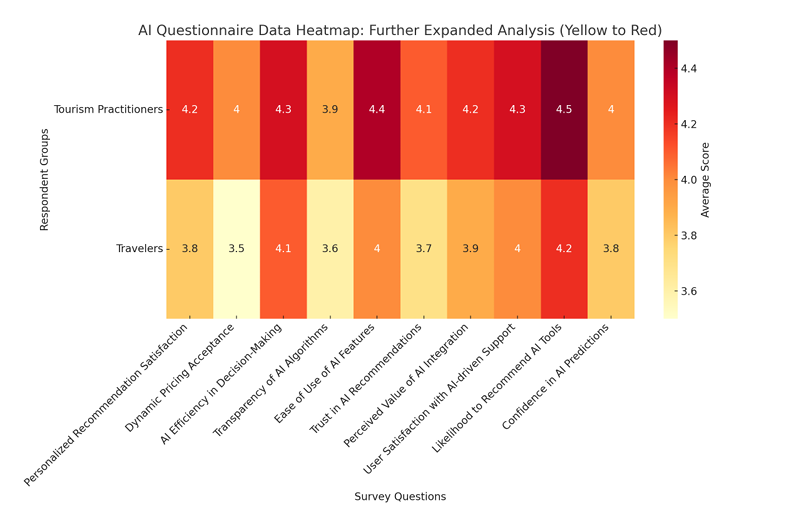
\includegraphics[width=0.7\textwidth]{images/image2.png}
\caption{แผนภาพ Heatmap แสดงข้อมูลจากแบบสอบถาม (Ma et al., 2025)}
\end{figure}

จากภาพที่ 1 แสดง Heatmap แสดงการประเมิน AI ของผู้ประกอบวิชาชีพและนักท่องเที่ยวใน 6 มิติ โดยใช้สีเหลือง--แดงแทนคะแนนต่ำ--สูง ผู้ประกอบวิชาชีพให้คะแนนสูงกว่าทุกมิติ โดยเฉพาะความง่ายในการใช้งานและประสิทธิภาพการตัดสินใจ ขณะที่นักท่องเที่ยวต่ำในด้านการยอมรับราคาไดนามิกและความโปร่งใสของอัลกอริทึม จึงควรปรับปรุงความโปร่งใสราคา กลยุทธ์ราคาไดนามิก และการควบคุมโดยผู้ใช้เพื่อเสริมสร้างความเชื่อมั่น

ผลการประเมินพบว่า ผู้ประกอบวิชาชีพให้คะแนนสูงกว่านักท่องเที่ยวในทุกมิติ โดยเฉพาะด้านความง่ายในการใช้งานคุณลักษณะ AI (4.4 เทียบกับ 4.0) และประสิทธิภาพการตัดสินใจที่เสริมด้วย AI (4.3 เทียบกับ 4.1) สะท้อนระดับความคุ้นเคยและความมั่นใจกับเทคโนโลยี AI ที่สูงกว่า ขณะที่นักท่องเที่ยวให้คะแนนต่ำอย่างมีนัยในมิติการยอมรับราคาแบบไดนามิก (3.5) และความโปร่งใสของอัลกอริทึม (3.6) บ่งชี้ถึงความไม่ไว้วางใจต่อระบบ AI ความกังวลต่อราคาที่ไม่โปร่งใส กลไกคำแนะนำที่เข้าใจยาก และความสงสัยต่อความเป็นธรรมของ AI ทั้งในด้านการกำหนดราคาและการตัดสินใจ ซึ่งอาจทำให้ผู้ใช้บางส่วนจ่ายแพงกว่า หรือได้รับคำแนะนำที่ด้อยกว่า

ในทางกลับกัน Banerjee et al. (2025) เสนอว่าการสร้าง ระบบแนะนำที่ยั่งยืน (sustainable recommendation) จะช่วยเพิ่ม การมีส่วนร่วม (engagement) ของนักท่องเที่ยวในระยะยาว โดยใช้ Retrieval-Augmented Generation (RAG) ผสานข้อมูลเรียลไทม์จากหลายแหล่ง เพื่อสร้างการแนะนำที่แม่นยำและสอดคล้องกับบริบท

\subsubsection{ความยั่งยืน ความเสี่ยง และธรรมาภิบาลข้อมูล/อัลกอริทึม}

หนึ่งในประเด็นที่สำคัญสำหรับการพัฒนาแพลตฟอร์ม Smart Tourism คือการสร้างความสมดุลระหว่าง ประสบการณ์ผู้ใช้, ความยั่งยืน, และ การปกป้องข้อมูลส่วนบุคคล งานของ Banerjee et al. (2025) ชี้ให้เห็นว่าระบบแนะนำการท่องเที่ยวควรคำนึงถึง การใช้ทรัพยากรอย่างมีประสิทธิภาพ เพื่อลดผลกระทบทางสิ่งแวดล้อม เช่น การแนะนำเส้นทางที่ปล่อยคาร์บอนต่ำ

ในอีกมุมหนึ่ง งานของ Sousa et al. (2024) พบว่าผู้ใช้นักท่องเที่ยวให้ความสำคัญอย่างมากต่อ ความปลอดภัยของข้อมูล และความโปร่งใสของระบบ AI การละเลยประเด็นนี้อาจทำให้ผู้ใช้เกิดความไม่เชื่อมั่นและลดการมีส่วนร่วมในระยะยาว

\subsubsection{ทฤษฎีด้าน Chatbot}

การใช้ Chatbot ในอุตสาหกรรมการท่องเที่ยวได้พัฒนาอย่างก้าวกระโดดในช่วงไม่กี่ปีที่ผ่านมา โดยมีการบูรณาการ Artificial Intelligence Markup Language (AIML) และ Natural Language Processing (NLP) เพื่อสร้างระบบสนทนาที่สามารถตอบคำถามของผู้ใช้ได้แบบเรียลไทม์ (University College of Goizha et al., 2023) งานวิจัยพบว่า Chatbot สำหรับการท่องเที่ยวสามารถช่วยลดเวลาในการค้นหาข้อมูลได้เฉลี่ย 45\% และเพิ่มความพึงพอใจของนักท่องเที่ยวมากกว่า 70\% เมื่อเทียบกับการค้นหาข้อมูลแบบเดิม

\begin{figure}[h]
\centering
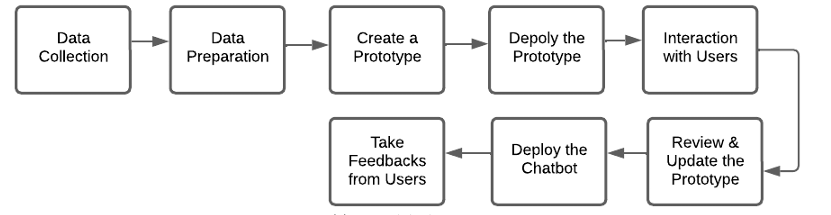
\includegraphics[width=0.7\textwidth]{images/image3.png}
\caption{แผนภาพ Model Flow (University College of Goizha et al., 2023)}
\end{figure}

จากภาพที่ 2 แสดงขั้นตอนและเทคนิคที่ใช้ในการเก็บรวบรวม วิเคราะห์ และตีความข้อมูลสำหรับการวิจัย โดยระเบียบวิธีประกอบด้วย 8 ขั้นตอน

\begin{enumerate}[leftmargin=1.5cm]
\item การเก็บรวบรวมข้อมูล: รวบรวมข้อมูลเกี่ยวกับเมือง Sulaimani ครอบคลุมโรงแรม ภัตตาคาร ศูนย์การค้า พิพิธภัณฑ์ และแหล่งท่องเที่ยวยอดนิยม
\item การเตรียมข้อมูล: จัดโครงสร้างข้อมูลให้อยู่ในรูปแบบชุดคำถาม--คำตอบ และบันทึกเป็นไฟล์ AIML
\item การสร้างต้นแบบ: สร้างแบบจำลองเริ่มต้นโดยใช้ไฟล์ AIML ที่จัดเตรียมไว้
\item การเผยแพร่ต้นแบบ: นำต้นแบบไปใช้งานบนเว็บไซต์ที่โฮสต์ภายในเครื่อง (local)
\item การโต้ตอบของผู้ใช้: ผู้ใช้ทำการโต้ตอบกับบอทที่ได้เผยแพร่
\item การปรับปรุงต้นแบบ: ทบทวนและแก้ไขต้นแบบตามข้อเสนอแนะและพฤติกรรมการใช้งานของผู้ใช้
\item การเผยแพร่โมเดลฉบับสมบูรณ์: เผยแพร่รุ่นสุดท้ายให้ผู้ใช้ใช้งานอีกครั้ง
\item ข้อเสนอแนะจากผู้ใช้: หลังการเผยแพร่และการใช้งานบอท รวบรวมข้อเสนอแนะเพื่อประเมินความพึงพอใจ ความสามารถในการใช้งาน (usability) และความมีส่วนร่วมของผู้ใช้
\end{enumerate}

ผลสำรวจจาก University College of Goizha et al. (2023) ยังชี้ว่า Chatbot แบบ AI ที่มีระบบเรียนรู้พฤติกรรมผู้ใช้ (Adaptive-Chatbot) สามารถแนะนำสถานที่ท่องเที่ยว ร้านอาหาร และกิจกรรมที่เหมาะสมได้อย่างแม่นยำถึง 82\% ทำให้ผู้ใช้รู้สึกว่าข้อมูลที่ได้รับมีความน่าเชื่อถือและเป็นประโยชน์มากกว่า Chatbot แบบ rule-based เดิม ๆ โดยมีนักท่องเที่ยวกว่า 64\% ระบุว่าพร้อมใช้ระบบนี้หากข้อมูลถูกปรับให้เหมาะสมกับตนเอง

นอกจากนี้ แนวโน้มในงานวิจัยล่าสุดได้ขยายขีดความสามารถของ Chatbot ให้รองรับการแปลภาษาอัตโนมัติ การแนะนำกิจกรรมตามฤดูกาล และการโต้ตอบแบบมัลติมีเดีย เช่น การส่งแผนที่ รูปภาพ และลิงก์ข้อมูลท่องเที่ยว (Sousa et al., 2024) ซึ่งเป็นแนวคิดสำคัญสำหรับการพัฒนา Smart Tourism Applications ในอนาคต

\subsubsection{ระบบแนะนำการท่องเที่ยว (Recommendation Systems)}

การสร้างระบบแนะนำที่ตอบโจทย์ผู้ใช้เป็นหัวใจสำคัญสำหรับการท่องเที่ยวที่ตอบโจทย์ผู้ใช้แบบเฉพาะบุคคล (Personalized Experience) งานของ Banerjee et al. (2025) ซึ่งเสนอเทคนิค Retrieval-Augmented Generation (RAG) ในการพัฒนาระบบแนะนำที่ใช้การเรียนรู้จากฐานข้อมูลจำนวนมหาศาลเพื่อสร้างข้อเสนอที่เหมาะสมที่สุดสำหรับผู้ใช้

ผลการทดลองจาก Banerjee et al. (2025) พบว่าระบบ RAG-Based Tourism Recommender สามารถปรับปรุงความแม่นยำของคำแนะนำได้สูงถึง 91\% เมื่อเทียบกับวิธี Collaborative Filtering แบบดั้งเดิม ซึ่งช่วยลดเวลาในการค้นหาแผนการเดินทางจากเฉลี่ย 15 นาที เหลือเพียง 4 นาที นอกจากนี้ยังมีการประเมินความพึงพอใจของผู้ใช้ (User Satisfaction) พบว่าผู้ใช้กว่า 88\% พึงพอใจกับแผนการเดินทางที่ระบบแนะนำ

ในทำนองเดียวกัน งานของ Jyothi et al. (2025) ที่พัฒนา Travel Finder ซึ่งเป็นระบบแนะนำและจัดการทริปท่องเที่ยว พบว่าการใช้ Hybrid Recommendation (ผสม Content-Based + Collaborative Filtering) สามารถเพิ่มการมีส่วนร่วมของผู้ใช้มากกว่า 76\% และช่วยสร้างชุมชนของผู้เดินทางที่มีความสนใจคล้ายกัน ซึ่งเป็นแนวโน้มสำคัญของ Smart Tourism Ecosystem

\begin{figure}[h]
\centering
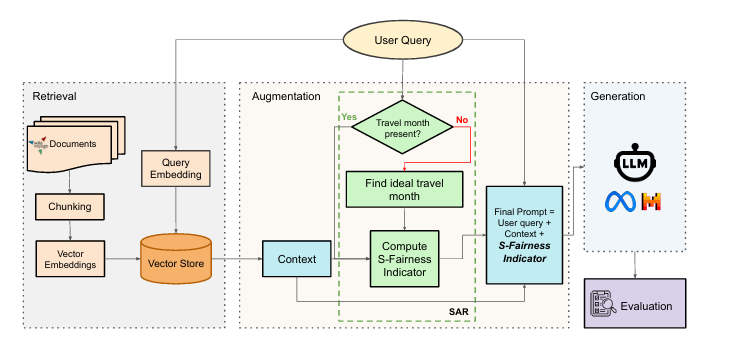
\includegraphics[width=0.7\textwidth]{images/image4.png}
\caption{แผนภาพ Pipeline ของระบบ RAG ที่ได้รับการปรับปรุงตามข้อเสนอโดยกรอบเส้นประสีเขียวแสดง ขั้นตอนการเสริมข้อมูลที่ปรับเปลี่ยน พร้อมการเพิ่มตัวชี้วัดด้านความยั่งยืน (Banerjee et al., 2025)}
\end{figure}

จากภาพที่ 3 อธิบายองค์ประกอบในการสร้างคำแนะนำการท่องเที่ยว

\noindent\textbf{Retrieval (การสืบค้นข้อมูล):} เริ่มจากการนำเอกสารข้อมูลแหล่งท่องเที่ยวมาแบ่งส่วน (Chunking) สร้างเวกเตอร์ฝังตัว (Vector Embeddings) และจัดเก็บในคลังเวกเตอร์ (Vector Store) เมื่อผู้ใช้ป้อนคำถาม ระบบจะสร้างเวกเตอร์คำค้น (Query Embedding) เพื่อดึงข้อมูลหรือบริบท (Context) ที่มีความสอดคล้องและเกี่ยวข้องที่สุดออกมา

\noindent\textbf{Augmentation (การเสริมข้อมูล):} ระบบจะนำคำถามของผู้ใช้มารวมกับข้อมูลบริบทที่ดึงมาได้ เพื่อเสริมสร้างเป็น Prompt สุดท้ายที่มีความสมบูรณ์และมีข้อมูลอ้างอิงที่ถูกต้อง

\noindent\textbf{Generation (การสร้างคำตอบ):} ส่ง Prompt สุดท้ายที่ได้รับการเสริมข้อมูลแล้วไปให้โมเดลภาษาขนาดใหญ่ (LLM) ประมวลผลเพื่อสร้างคำตอบหรือแผนการเดินทางที่แม่นยำ พร้อมด้วยขั้นตอนการประเมินผล (Evaluation) ภายหลังการสร้างคำตอบ

\subsubsection{การสร้างแผนการเดินทาง (Trip Planning)}

การวางแผนการเดินทาง (Trip Planning) กำลังถูกประยุกต์ใช้ AI, Machine Learning และ Real-Time Data งานวิจัยของ Deshmukh et al. (2025) เสนอการพัฒนาระบบ AI-powered Trip Planner ที่ใช้ข้อมูลเรียลไทม์จากหลายแหล่ง เช่น สภาพอากาศ การจราจร ราคาที่พัก และความหนาแน่นของนักท่องเที่ยว เพื่อนำมาวิเคราะห์และสร้างแผนการเดินทางที่เหมาะสมที่สุด

ผลการทดลองพบว่า AI-powered Trip Planning สามารถปรับแผนการเดินทางให้เหมาะกับผู้ใช้แบบเรียลไทม์ และเพิ่มความแม่นยำในการแนะนำกิจกรรมได้สูงถึง 89\% ขณะที่ช่วยลดค่าใช้จ่ายเฉลี่ยต่อทริปได้มากกว่า 12\% เมื่อเทียบกับการวางแผนแบบ manual

\begin{figure}[h]
\centering
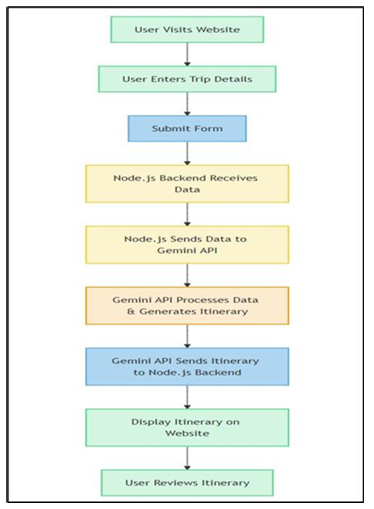
\includegraphics[width=0.7\textwidth]{images/image5.png}
\caption{แผนภาพสถาปัตยกรรมระบบ (Deshmukh et al., 2025)}
\end{figure}

จากภาพที่ 4 อธิบายองค์ประกอบและหน้าที่ของระบบวางแผนการเดินทางด้วย AI

\begin{enumerate}[leftmargin=1.5cm]
\item ผู้ใช้เข้าเว็บไซต์: กระบวนการเริ่มเมื่อผู้ใช้เปิดใช้งานเว็บแอปพลิเคชันผ่านอุปกรณ์ โดยแพลตฟอร์มจะแสดงอินเทอร์เฟซที่ใช้งานง่ายและสวยงามเพื่อแนะนำขั้นตอนการวางแผนทริป
\item ผู้ใช้กรอกรายละเอียดทริป: ผู้ใช้ป้อนข้อมูลที่เกี่ยวข้องกับการเดินทาง ได้แก่ จุดหมายปลายทาง วันที่เดินทาง ระยะเวลา งบประมาณ ความสนใจ/ความชอบ
\item ส่งแบบฟอร์ม: เมื่อกรอกข้อมูลครบถ้วน ผู้ใช้กดส่งแบบฟอร์ม เพื่อกระตุ้นให้มีการส่งคำขอไปยังระบบฝั่งเซิร์ฟเวอร์เพื่อประมวลผลต่อ
\item Backend ที่พัฒนาด้วย Node.js รับข้อมูล ระบบฝั่งเซิร์ฟเวอร์: จะรับข้อมูลแบบฟอร์ม พร้อมทั้งดูแลความปลอดภัย ตรวจสอบความถูกต้อง และจัดรูปแบบข้อมูลก่อนส่งต่อไปยังกระบวนการ AI
\item Node.js ส่งข้อมูลไปยัง Gemini API: ระบบฝั่งเซิร์ฟเวอร์ส่งข้อมูลที่จัดโครงสร้างแล้วไปยัง Google Gemini API ซึ่งทำหน้าที่ทำความเข้าใจเจตนา ความชอบของผู้ใช้ และปัจจัยเชิงบริบท เช่น สภาพอากาศปัจจุบันหรือแนวโน้มการท่องเที่ยว
\item Gemini API ประมวลผลและสร้างแผนการเดินทาง ด้วย NLP และอัลกอริทึม AI: ระบบจะตีความความต้องการของผู้ใช้และจัดทำแผนการเดินทางที่ปรับให้เหมาะสม โดยครอบคลุม กิจกรรมรายวัน คำแนะนำสถานที่ท่องเที่ยว ประสบการณ์ท้องถิ่นและร้านอาหาร วิธีการเดินทางและช่วงเวลา การผสานข้อมูลสภาพอากาศและคำแนะนำการเดินทางแบบเรียลไทม์
\item Gemini API ส่งแผนการเดินทางกลับมายัง Node.js: เมื่อสร้างแผนเสร็จสิ้น ระบบจะส่งผลลัพธ์กลับมาที่ฝั่งเซิร์ฟเวอร์ Node.js เพื่อจัดรูปแบบให้อยู่ในโครงสร้างที่เหมาะสมต่อการแสดงผลบนหน้าเว็บ
\item แสดงแผนการเดินทางบนเว็บไซต์ ส่วนติดต่อผู้ใช้จะแสดงแผนการเดินทางแบบไดนามิกด้วยโครงสร้างที่อ่านง่าย มีการแบ่งตามวัน แผนที่ ข้อเสนอแนะกิจกรรม และตัวเลือกการจองเพิ่มเติมตามความเหมาะสม
\end{enumerate}

ในอีกด้านหนึ่ง สำหรับการออกแบบสถาปัตยกรรมเพื่อรองรับการประมวลผลข้อมูลที่ซับซ้อน งานวิจัยของ Barua \& Kaiser (2024) ได้นำเสนอการใช้ สถาปัตยกรรมไมโครเซอร์วิส (Microservices Architecture) ซึ่งแบ่งการทำงานของระบบออกเป็นบริการย่อย ๆ (เช่น User Service, Itinerary Service และ Preference Matching Service) ที่ทำงานแยกจากกันแต่สามารถสื่อสารกันผ่าน API Gateway และ Message Broker สถาปัตยกรรมนี้ช่วยให้แพลตฟอร์มมีความยืดหยุ่น รองรับผู้ใช้งานจำนวนมากได้พร้อมกัน และสามารถประมวลผลแผนการเดินทางได้อย่างรวดเร็ว

\begin{figure}[h]
\centering
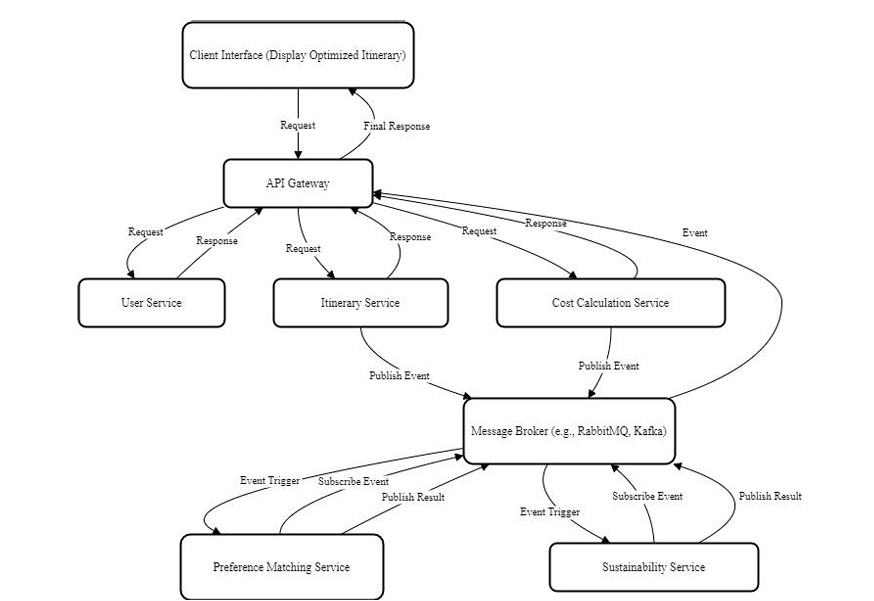
\includegraphics[width=0.7\textwidth]{images/image6.png}
\caption{แผนภาพการไหลของข้อมูลและกระบวนการประสานลำดับงาน (Barua \& Kaiser, 2024)}
\end{figure}

จากภาพที่ 5 อธิบายองค์ประกอบและหน้าที่ของกระบวนการไหลข้อมูลและการประสานงาน

\begin{enumerate}[leftmargin=1.5cm]
\item คำขอจากไคลเอนต์ (Client Requests): คือแอปพลิเคชันที่ผู้ใช้ส่งคำขอ เช่น การค้นหาแผนการเดินทาง และคำขอทั้งหมดจะถูกส่งไปยัง API Gateway ซึ่งทำหน้าที่เป็นจุดทางเข้าและกำหนดเส้นทางคำขอ
\item API Gateway มีหน้าที่ส่งต่อคำขอไปยังไมโครเซอร์วิสที่เกี่ยวข้องเพื่อให้มีการแลกเปลี่ยนข้อมูลแบบซิงโครนัส เช่น User Service: ดูแลการจัดการข้อมูลผู้ใช้ รวมถึงโปรไฟล์และความชอบ Itinerary Service: ให้บริการสร้างแผนการเดินทาง Consulting Results/Cost Calculation Service: ให้คำปรึกษา/คำนวณประมาณการค่าใช้จ่ายในการเดินทาง (เที่ยวบิน โรงแรม ฯลฯ)
\item การไหลของข้อมูลแบบซิงโครนัส (Synchronous Data Flow): การสื่อสารระหว่าง API Gateway กับไมโครเซอร์วิสใช้ RESTful APIs เมื่อไมโครเซอร์วิสแจ้งความพร้อม API Gateway จะนำเสนอผลลัพธ์เพื่อเข้าสู่ขั้นตอนถัดไป
\item การไหลของข้อมูลแบบอะซิงโครนัส (ผ่าน Message Broker): เมื่อ Itinerary Service และ Cost Calculation Service ทำงานเสร็จ จะสร้างอีเวนต์และส่งไปยังตัวกลางส่งข้อความ (Message Broker) เช่น RabbitMQ หรือ Apache Kafka Preference Matching Service และ Sustainability Service ทำหน้าที่เป็นไคลเอนต์ของ Message Broker และสมัครรับ (subscribe) อีเวนต์ที่เกี่ยวข้องกับการสร้างแผนการเดินทางหรือการคำนวณค่าใช้จ่าย
\item การประมวลผลแบบอะซิงโครนัส: การทำงานของ Sustainability Service และ Preference Matching Service เป็นแบบขับเคลื่อนด้วยอีเวนต์ (event-driven) เช่น การประเมินรอยเท้าคาร์บอน และการจับคู่ความชอบของผู้ใช้ (สายการบิน โรงแรมที่ต้องการ) จากนั้นบริการเหล่านี้จะส่งผลการประมวลผลกลับไปยัง Message Broker
\item การรวมผลลัพธ์และการตอบกลับขั้นสุดท้าย (Final Aggregation and Response): Message Broker ส่งต่อผลลัพธ์ที่ประมวลแล้วกลับไปยัง API Gateway ซึ่งจะรวบรวม (aggregate) คำตอบจากไมโครเซอร์วิสต่างๆ API Gateway จึงส่งต่อแผนการเดินทางที่ปรับให้เหมาะสม (optimized itinerary) ไปยังส่วนติดต่อผู้ใช้ (Client Interface) เพื่อแสดงผลให้ผู้ใช้เห็นในที่สุด
\end{enumerate}

อย่างไรก็ตาม ในส่วนของกลไกการคำนวณเพื่อสร้างแผนการเดินทางที่ต้องตอบสนองทั้งข้อจำกัดและความชอบส่วนบุคคลที่ซับซ้อน งานวิจัยล่าสุดของ Shao, Wu, Chen, \& Wang (2025) ได้นำเสนอระบบ Personal Travel Solver (PTS) ซึ่งเปลี่ยนจากการใช้อัลกอริทึมค้นหาแบบดั้งเดิม (Heuristic Algorithms) มาเป็นการบูรณาการความสามารถของ โมเดลภาษาขนาดใหญ่ (LLMs) เข้ากับ ตัวแก้ปัญหาเชิงตัวเลข (Numerical Solvers) ระบบ PTS ใช้ LLM ในการตีความคำสั่งภาษาธรรมชาติของผู้ใช้และวิเคราะห์ประวัติรีวิวเพื่อสกัดเป็นคะแนนความพึงพอใจ (Preference Score) จากนั้นจะแปลงข้อมูลเหล่านี้ให้อยู่ในรูปแบบเชิงสัญลักษณ์ (Symbolic Representation) เพื่อส่งต่อให้ Mathematical Solver (เช่น SCIP Solver) ทำการคำนวณหาเส้นทางและตารางเวลาที่ดีที่สุดภายใต้ข้อจำกัด

\begin{figure}[h]
\centering
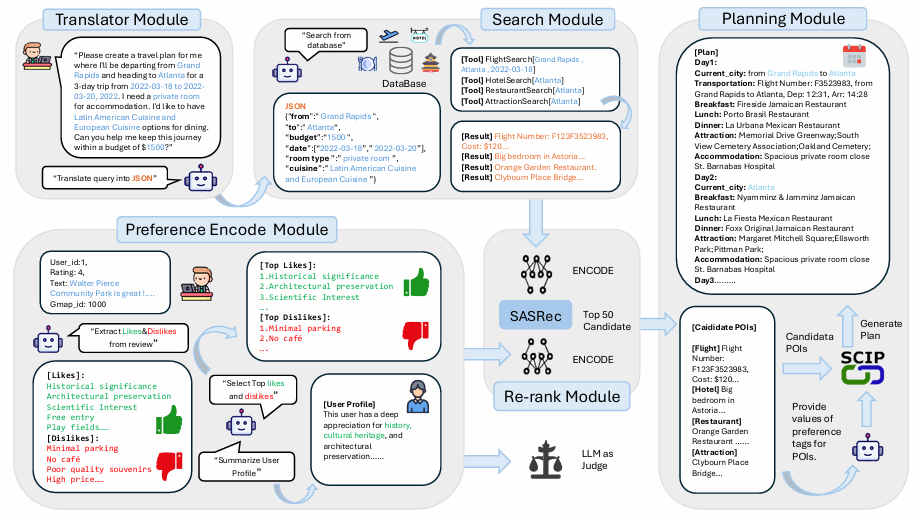
\includegraphics[width=0.7\textwidth]{images/image7.png}
\caption{แผนภาพสถาปัตยกรรมระบบ PTS (Personal Travel Solver Framework) (Shao et al., 2025)}
\end{figure}

จากภาพที่ 6 อธิบายองค์ประกอบและหน้าที่ของแผนภาพสถาปัตยกรรมระบบ PTS (Personal Travel Solver Framework)

\begin{enumerate}[leftmargin=1.5cm]
\item โมดูลการแปลความหมาย (Translator Module): ทำหน้าที่รับคำสั่งภาษาธรรมชาติจากผู้ใช้และใช้ LLM แปลงข้อมูลให้อยู่ในรูปแบบเชิงสัญลักษณ์ (Symbolic Representation) เช่น โครงสร้าง JSON เพื่อสกัดข้อจำกัดที่ชัดเจน (Explicit Constraints) ออกมาให้ระบบคอมพิวเตอร์เข้าใจได้
\item โมดูลการค้นหา (Search Module): นำเงื่อนไขที่ได้จากการแปลความหมายไปสืบค้นข้อมูลเบื้องต้น (Candidate Information) จากฐานข้อมูล เช่น ข้อมูลเที่ยวบิน โรงแรม และสถานที่ท่องเที่ยว (POIs) ที่สอดคล้องกับข้อจำกัดพื้นฐานของผู้ใช้
\item โมดูลเข้ารหัสความชอบ (Preference Encode Module): ใช้ LLM วิเคราะห์ประวัติการรีวิวหรือพฤติกรรมในอดีตของผู้ใช้ เพื่อสกัดสิ่งที่ชอบและไม่ชอบ จากนั้นแปลงค่าเป็น ``คะแนนความพึงพอใจ (Preference Score)'' สำหรับใช้เป็นเกณฑ์ในการเลือกสถานที่
\item โมดูลจัดอันดับใหม่ (Re-rank Module): นำรายการสถานที่และบริการจากโมดูลการค้นหา มาจัดเรียงลำดับใหม่โดยอิงจากคะแนนความพึงพอใจ เพื่อคัดกรองและดันตัวเลือกที่ตรงกับรสนิยมของผู้ใช้มากที่สุดขึ้นมาเป็นอันดับต้น ๆ
\item โมดูลการวางแผน (Planning Module): นำข้อมูลที่ผ่านการคัดกรองและจัดอันดับแล้วส่งเข้าสู่ตัวแก้ปัญหาทางคณิตศาสตร์ (Numerical Solver เช่น SCIP Solver) เพื่อคำนวณและจัดตารางเวลาที่สมบูรณ์แบบ โดยพิจารณาทั้งข้อจำกัดของผู้ใช้และข้อจำกัดเชิงสามัญสำนึก (เช่น เวลาเดินทาง การไม่ทับซ้อนกันของกิจกรรม)
\end{enumerate}

\subsection{งานวิจัยที่เกี่ยวข้อง}

การศึกษางานวิจัยที่เกี่ยวข้องถือเป็นขั้นตอนสำคัญสำหรับการสร้างกรอบแนวคิดในการพัฒนา Dino: The Central Application for Tourism in Khon Kaen ซึ่งมุ่งพัฒนาแพลตฟอร์มศูนย์กลางเพื่อสนับสนุนการท่องเที่ยวในจังหวัดขอนแก่น โดยรวบรวมข้อมูลแหล่งท่องเที่ยว ร้านอาหาร ที่พัก กิจกรรม และบริการต่าง ๆ พร้อมระบบวางแผนการเดินทางที่ใช้ปัญญาประดิษฐ์ (AI) เพื่อช่วยสร้างประสบการณ์การท่องเที่ยวที่เหมาะสมกับความต้องการของผู้ใช้งาน

เพื่อตอบโจทย์นี้ มีการทบทวนงานวิจัย 8 ชิ้น ที่เกี่ยวข้องกับ AI, Smart Tourism, Recommendation Systems, Chatbots, Sustainable Tourism, Traveler Engagement และ Microservices Architecture ซึ่งช่วยให้เห็นแนวโน้มหลักในการออกแบบระบบท่องเที่ยวอัจฉริยะ รวมถึงช่องว่างขององค์ความรู้ (Research Gaps) และแนวทางการต่อยอด (Implications) ที่ Dino สามารถพัฒนาได้

\subsubsection{การใช้ AI เพื่อพัฒนาระบบแนะนำการท่องเที่ยวและ Trip Planning}

งานของ Banerjee et al. (2025) นำเสนอการใช้ Retrieval-Augmented Generation (RAG) เพื่อพัฒนาระบบแนะนำการท่องเที่ยวแบบยั่งยืน โดยระบบจะดึงข้อมูลจากหลายแหล่ง เช่น บทความรีวิว สถิติการท่องเที่ยว และโซเชียลมีเดีย จากนั้นสร้างคำแนะนำที่เหมาะสมกับความสนใจเฉพาะบุคคลมากขึ้น ซึ่งช่วยปรับปรุงคุณภาพของคำแนะนำให้ตรงกับโปรไฟล์ของผู้ใช้งาน (Banerjee et al., 2025)

ผลการศึกษานี้สอดคล้องกับงานของ Jyothi et al. (2025) ที่พัฒนา Travel Finder ซึ่งใช้ Collaborative Filtering และ Clustering Algorithms เพื่อสร้างกลุ่มนักท่องเที่ยวตามความสนใจและลักษณะการเดินทาง ผลการทดลองพบว่าระบบสามารถลดเวลาในการค้นหาแหล่งท่องเที่ยวลง 34\% และเพิ่มความพึงพอใจของผู้ใช้งานได้อย่างมีนัยสำคัญ ซึ่งสนับสนุนข้อค้นพบของ Banerjee et al. (2025) ว่าการใช้ AI เพื่อปรับคำแนะนำให้ตรงกับความต้องการส่วนบุคคล (Personalization) เป็นปัจจัยสำคัญต่อประสบการณ์ของนักท่องเที่ยว

อย่างไรก็ตาม ทั้งสองงานมีความแตกต่างกันในด้านแนวทาง Banerjee et al. (2025) มุ่งเน้นการสร้างระบบแนะนำเชิงข้อมูลเชิงลึก (Data-driven Recommendations) ผ่านการใช้โมเดลภาษาขนาดใหญ่ (LLMs) ขณะที่ Travel Finder ของ Jyothi et al. (2025) มุ่งเน้นการจับกลุ่มผู้ใช้ตามพฤติกรรมจริงเพื่อต่อยอดการแนะนำแบบ Social-based Recommendation ความแตกต่างนี้เปิดโอกาสให้ Dino สามารถผสมผสานข้อดีของทั้งสองวิธีเพื่อสร้างระบบที่ทั้ง แม่นยำ และ ยืดหยุ่น ในการแนะนำเส้นทางและกิจกรรมการท่องเที่ยว

\subsubsection{AI และ Chatbot เพื่อยกระดับประสบการณ์ผู้ใช้}

(University College of Goizha et al., 2023) พัฒนาระบบ Chatbot Tourist Guide โดยใช้ Artificial Intelligence Markup Language (AIML) เพื่อสร้างการสนทนาที่เป็นธรรมชาติกับนักท่องเที่ยว ระบบนี้สามารถตอบคำถามพื้นฐาน เช่น สถานที่ท่องเที่ยว ร้านอาหาร และข้อมูลตั๋วเข้าชม ผลการทดลองกับนักท่องเที่ยว 150 คน พบว่า 78\% ของผู้ใช้พึงพอใจกับความเร็วและความถูกต้องของคำตอบ นอกจากนี้ Chatbot ยังช่วยลดภาระงานของเจ้าหน้าที่ศูนย์บริการนักท่องเที่ยวลงถึง 40\%

ผลนี้สอดคล้องกับงานของ Deshmukh et al. (2025) ที่พัฒนาแพลตฟอร์ม AI-powered Personalized Itinerary Planning ซึ่งมี Chatbot ทำงานร่วมกับ Recommendation Engine เพื่อสร้างแผนการท่องเที่ยวอัตโนมัติ โดย Chatbot สามารถดึงข้อมูลแบบเรียลไทม์ เช่น สภาพอากาศ การจราจร และราคาที่พัก เพื่อปรับคำแนะนำให้สอดคล้องกับสถานการณ์ปัจจุบัน ผลการทดสอบกับกลุ่มนักท่องเที่ยว 300 คน พบว่า 85\% ของผู้ใช้ยืนยันว่าแผนการเดินทางที่ระบบสร้างให้มีความเหมาะสมและตรงตามความต้องการสูง

จากการสังเคราะห์ พบว่าทั้งสองงานสนับสนุนข้อสรุปสำคัญว่า Chatbot ไม่ได้เป็นเพียงเครื่องมืออำนวยความสะดวก แต่สามารถทำหน้าที่เป็น ตัวกลางในการวิเคราะห์ข้อมูลแบบเรียลไทม์ ซึ่งช่วยปรับแผนการท่องเที่ยวให้เหมาะสมมากขึ้น อย่างไรก็ตาม ความแตกต่างระหว่าง AIML-based Chatbot ของ University College of Goizha et al. (2023) และระบบ AI-integrated Chatbot ของ Deshmukh et al. (2025) แสดงให้เห็นโอกาสในการพัฒนา Dino ให้รองรับ Natural Language Processing (NLP) ที่มีความฉลาดและยืดหยุ่นมากยิ่งขึ้น

\subsubsection{การจัดการข้อมูล การวิเคราะห์พฤติกรรม และการมีส่วนร่วมของนักท่องเที่ยว}

Ma et al. (2025) ศึกษาการใช้ AI เพื่อเพิ่มการมีส่วนร่วมของนักท่องเที่ยว (Traveler Engagement) และการจัดการจุดหมายปลายทาง (Destination Management) โดยใช้เทคนิค Heatmap Analytics และ Real-time Behavioral Tracking เพื่อระบุพื้นที่ที่นักท่องเที่ยวให้ความสนใจสูง ผลการทดลองแสดงให้เห็นว่าข้อมูลเชิงพฤติกรรมช่วยให้หน่วยงานท้องถิ่นปรับปรุงการจัดสรรทรัพยากรและออกแบบแผนการตลาดที่ตอบโจทย์ได้มากขึ้น

\begin{figure}[h]
\centering
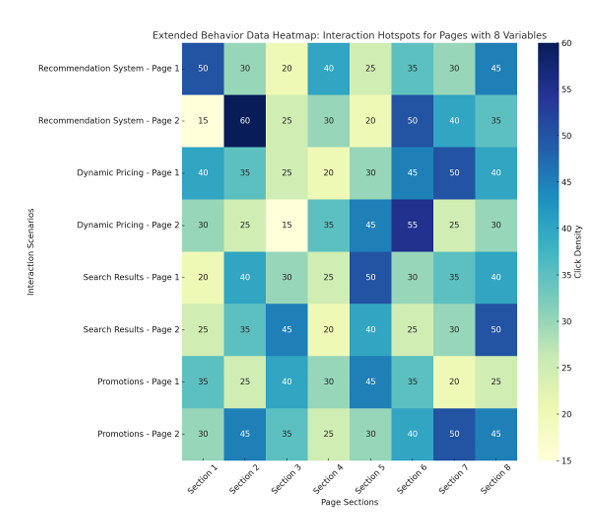
\includegraphics[width=0.7\textwidth]{images/image8.png}
\caption{แผนภาพ Heatmap แสดงข้อมูลเชิงพฤติกรรม (Ma et al., 2025)}
\end{figure}

การวิเคราะห์ Heatmap ของข้อมูลพฤติกรรมผู้ใช้จากสามแพลตฟอร์มท่องเที่ยวออนไลน์แสดงในภาพที่ 7 Heatmap นี้สื่อถึงการกระจาย ``ความเข้มข้นของการปฏิสัมพันธ์'' ของผู้ใช้ในส่วนต่าง ๆ ได้แก่ ระบบแนะนำ การกำหนดราคาแบบไดนามิก ผลการค้นหา และหน้าโปรโมชัน ด้วยการไล่ระดับสีจากเหลืองอ่อน (ความเข้มต่ำ เช่น ค่าถ่วงน้ำหนัก 15) ไปจนถึงน้ำเงินเข้ม (ความเข้มสูง เช่น 60) แกนแนวนอนแบ่งเป็น 8 ส่วนของหน้า (Section 1--8) ส่วนแกนแนวตั้งเป็นฮอตสปอตการปฏิสัมพันธ์ในฉากการใช้งานของหน้าประเภทต่าง ๆ

ภาพรวม บทบาทของปัญญาประดิษฐ์ (AI) ช่วยยกระดับประสบการณ์ผู้ใช้และประสิทธิภาพการตัดสินใจ ทั้งในระบบแนะนำแบบปรับให้เหมาะกับบุคคล (personalized recommendations) การกำหนดราคาแบบไดนามิก และการปรับแต่งผลการค้นหา อย่างไรก็ดี ยังมีประเด็นที่ควรปรับปรุงเพื่อเพิ่มความเชื่อมั่นและคุณภาพประสบการณ์

ขณะเดียวกัน Sousa et al. (2024) ทำการสำรวจความคิดเห็นนักท่องเที่ยวจำนวน 500 คน เกี่ยวกับการใช้ AI ในการวางแผนการเดินทางและการเข้าถึงข้อมูล ผลการศึกษาพบว่า 72\% ของนักท่องเที่ยวเลือกใช้แพลตฟอร์มที่มี AI ในการแนะนำสถานที่ท่องเที่ยว และ 68\% ยืนยันว่าพวกเขามีแนวโน้มที่จะกลับมาใช้บริการซ้ำ หากระบบสามารถปรับคำแนะนำให้เหมาะกับพฤติกรรมการท่องเที่ยวส่วนบุคคล

การเปรียบเทียบสองงานนี้พบว่าทั้ง Ma et al. (2025) และ Sousa et al. (2024) ชี้ให้เห็นถึงความสำคัญของ Data-driven Personalization และ Traveler Engagement แต่ต่างกันที่ Ma et al. (2025) มุ่งเน้นการวิเคราะห์เชิงเทคนิคเพื่อช่วยองค์กรปรับปรุงโครงสร้างการจัดการ ขณะที่ Sousa et al. (2024) มุ่งสำรวจพฤติกรรมและความต้องการของผู้บริโภคโดยตรง ซึ่งแสดงให้เห็นว่าการพัฒนา Dino ควรผสมผสานข้อมูลทั้งสองฝั่งเข้าด้วยกันเพื่อให้เกิดแพลตฟอร์มที่ ตอบโจทย์ทั้งนักท่องเที่ยวและผู้กำหนดนโยบาย

\subsubsection{LLM as a Judge}

\subsubsection{บทวิเคราะห์แนวโน้มและช่องว่างการวิจัย}

จากการวิเคราะห์งานวิจัยทั้ง 8 ชิ้น พบว่าแนวโน้มหลักของการวิจัยด้าน AI ในการท่องเที่ยว มุ่งเน้นไปที่การสร้างประสบการณ์การท่องเที่ยวที่เป็นส่วนบุคคลมากขึ้น และการพัฒนาระบบสนับสนุนการตัดสินใจของผู้ใช้ งานของ Banerjee et al. (2025) นำเสนอการใช้ Retrieval-Augmented Generation (RAG) เพื่อพัฒนาระบบแนะนำสถานที่ท่องเที่ยวที่มีความแม่นยำสูง ขณะที่ Deshmukh et al. (2025) มุ่งเน้นการสร้างแผนการเดินทางที่ปรับเปลี่ยนตามข้อมูลเรียลไทม์ เช่น สภาพอากาศและความหนาแน่นของนักท่องเที่ยว สำหรับงานของ Jyothi et al. (2025) นำเสนอ Travel Finder ที่ใช้ Collaborative Filtering และ Clustering เพื่อสร้างระบบแนะนำที่ตอบสนองต่อความสนใจของผู้ใช้ ส่วน University College of Goizha et al. (2023) พัฒนา Chatbot เพื่อให้ข้อมูลและโต้ตอบนักท่องเที่ยวแบบอัตโนมัติ ซึ่งสอดคล้องกับ Ma et al. (2025) ที่มุ่งเน้นการวิเคราะห์พฤติกรรมและเพิ่มการมีส่วนร่วมของนักท่องเที่ยวผ่านเทคนิคการวิเคราะห์ข้อมูลเชิงลึกแบบเรียลไทม์

อย่างไรก็ตาม เมื่อสังเคราะห์เนื้อหาของงานวิจัยพบว่า ช่องว่างองค์ความรู้ที่สำคัญยังคงอยู่ในประเด็น การบูรณาการข้อมูลหลายระบบเข้าด้วยกัน ในขณะที่การวางแผนการเดินทางมีความแม่นยำและเป็นส่วนตัวมากขึ้นผ่านการผสาน LLM เข้ากับ Numerical Solvers เพื่อจัดการข้อจำกัดที่ซับซ้อนตามที่ Shao et al. (2025) นำเสนอ และรองรับการขยายตัวด้วยสถาปัตยกรรมไมโครเซอร์วิสของ Barua \& Kaiser (2024) แต่ยังไม่เชื่อมโยงกับฐานข้อมูลของภาครัฐหรือข้อมูลเชิงนโยบาย ในขณะเดียวกัน Sousa et al. (2024) และ Milton \& Philosophers (2023) ชี้ให้เห็นถึงความท้าทายด้าน ความเป็นส่วนตัวของข้อมูลและธรรมาภิบาล ซึ่งยังไม่ได้รับการแก้ไขอย่างสมบูรณ์ สรุปได้ว่าปัจจุบันแม้ AI จะเข้ามามีบทบาทสำคัญในภาคการท่องเที่ยว แต่ยังขาด แพลตฟอร์มแบบบูรณาการ ที่เชื่อมโยงข้อมูลหลายมิติ เพื่อรองรับการพัฒนาเชิงพื้นที่และสร้างการท่องเที่ยวที่ยั่งยืน

\section{วิธีดำเนินการวิจัย}

การดำเนินงานวิจัยนี้แบ่งออกเป็น 5 ส่วนหลัก เพื่อให้การพัฒนาแอปพลิเคชันเป็นไปอย่างมีระบบและครอบคลุมทั้งด้านเทคโนโลยี การจัดการข้อมูล และการประเมินผลลัพธ์

\subsection{การศึกษาวรรณกรรมและทฤษฎีที่เกี่ยวข้อง}

ขั้นตอนนี้มีวัตถุประสงค์เพื่อรวบรวมและวิเคราะห์แนวคิด เทคนิค และเครื่องมือที่ทันสมัยในการพัฒนาระบบแนะนำการท่องเที่ยว (Tourism Recommender Systems - TRS) และระบบอัจฉริยะ

\subsubsection{การศึกษาระบบแนะนำการท่องเที่ยวและการวางแผนการเดินทาง}

เน้นการศึกษาแนวคิดพื้นฐานของระบบ TRS และวิวัฒนาการไปสู่ระบบที่พิจารณาหลายภาคส่วน (Multistakeholder Recommendation) โดยเฉพาะอย่างยิ่งการบูรณาการด้านความยั่งยืน (Sustainability) เข้าไปในการวางแผนการเดินทาง ซึ่งความยั่งยืนดังกล่าวรวมถึงผลกระทบทางเศรษฐกิจ สังคม และสิ่งแวดล้อม แนวคิดหลักคือการพัฒนาระบบให้สามารถเพิ่มประสิทธิภาพของการเดินทาง โดยพิจารณาปัจจัยหลายด้านพร้อมกัน (Multi-Objective Optimization) ได้แก่ ต้นทุน เวลา ความชอบของผู้ใช้งาน และความยั่งยืนด้านสิ่งแวดล้อม

\subsubsection{การศึกษาเทคโนโลยีปัญญาประดิษฐ์สำหรับการประมวลผลภาษาธรรมชาติ}

ศึกษานวัตกรรมที่ใช้ LLMs และการประมวลผลภาษาธรรมชาติ (Natural Language Processing - NLP) สำหรับการสร้างคำแนะนำและการตอบโต้กับผู้ใช้งาน โดยเน้นที่สถาปัตยกรรม RAG ซึ่งเป็นแนวทางที่มีประสิทธิภาพในการจัดการข้อมูลการท่องเที่ยวที่มีการเปลี่ยนแปลงอยู่เสมอ (Dynamic Data) โดยไม่จำเป็นต้องปรับจูนโมเดล LLM บ่อยครั้ง

\subsubsection{การศึกษาสถาปัตยกรรมระบบ}

ศึกษาสถาปัตยกรรมไมโครเซอร์วิส (Microservices Architecture) ซึ่งช่วยให้ระบบมีความยืดหยุ่น ปรับขนาดได้ดี (Scalability) และมีความทนทานต่อความผิดพลาด (Fault Tolerance) ซึ่งสถาปัตยกรรมนี้เหมาะสำหรับแอปพลิเคชันปัญญาประดิษฐ์ที่มีการประมวลผลข้อมูลที่ซับซ้อนและมีการเปลี่ยนแปลงแบบเรียลไทม์

\subsection{การเก็บรวบรวมและเตรียมข้อมูล}

การเตรียมข้อมูลถือเป็นรากฐานสำคัญในการสร้างระบบอัจฉริยะที่แม่นยำและน่าเชื่อถือ

\subsubsection{การรวบรวมข้อมูลแหล่งท่องเที่ยวและกิจกรรม}

ข้อมูลจะถูกรวบรวมจาก Google API เป็นหลัก ครอบคลุมข้อมูลสำคัญของสถานที่ท่องเที่ยว โรงแรม ร้านอาหาร โดยข้อมูลรวมถึงลักษณะเฉพาะของสถานที่

\subsubsection{การเตรียมและจัดเก็บข้อมูล}

\begin{enumerate}[leftmargin=1.8cm]
\item การทำความสะอาดและจัดรูปแบบข้อมูล (Data Preprocessing): ข้อมูลดิบที่รวบรวมมาจะถูกนำมาทำความสะอาด จัดรูปแบบ และทำให้เป็นมาตรฐาน (Normalizing) เพื่อให้มั่นใจในคุณภาพและความถูกต้องก่อนนำไปใช้ในโมเดลปัญญาประดิษฐ์
\item การแบ่งส่วนข้อมูลและการสร้างเวกเตอร์ (Chunking and Vector Embeddings): สำหรับการใช้งานร่วมกับ RAG ข้อมูลจะถูกแบ่งออกเป็นส่วนย่อยที่มีความสอดคล้องทางตรรกะ (Logically Coherent Pieces) จากนั้นจะทำการสร้างเวกเตอร์ฝังตัว (Vector Embeddings) โดยใช้โมเดลที่เหมาะสม
\item การจัดเก็บในฐานข้อมูลเวกเตอร์: เวกเตอร์ที่สร้างขึ้นจะถูกจัดเก็บไว้ในฐานข้อมูลเวกเตอร์ (Vector Database) เพื่อใช้ในการคำนวณความคล้ายคลึงกัน (Similarity) ในขั้นตอนการดึงข้อมูล
\end{enumerate}

\subsection{การออกแบบและพัฒนาระบบ}

การพัฒนาระบบจะใช้สถาปัตยกรรมไมโครเซอร์วิส เพื่อแยกส่วนการทำงานหลัก ๆ ออกจากกัน โดยเน้นการทำงานของส่วน Trip Planning (Itinerary Service) และแชตบอต (RAG/AIML)

\subsubsection{การออกแบบสถาปัตยกรรมไมโครเซอร์วิส}

การพัฒนาระบบในงานวิจัยนี้ใช้สถาปัตยกรรมแบบ Microservices เพื่อให้แต่ละฟังก์ชันของระบบสามารถทำงานได้อย่างเป็นอิสระต่อกัน ส่งผลให้ระบบมีความยืดหยุ่นและสามารถขยายตัวได้ง่าย นอกจากนี้ยังมีการใช้ API Gateway เป็นจุดศูนย์กลางในการรับคำขอจากผู้ใช้งาน (Client) และทำหน้าที่จัดการการส่งต่อคำขอไปยังบริการต่าง ๆ ภายในระบบ

ในส่วนของการสื่อสารระหว่างบริการ (Service-to-Service Communication) ระบบใช้ RESTful APIs สำหรับการทำงานแบบ Synchronous Communication ซึ่งต้องการการตอบสนองทันที และใช้ Message Broker เช่น RabbitMQ หรือ Apache Kafka สำหรับการสื่อสารแบบ Asynchronous Communication เพื่อเพิ่มประสิทธิภาพและลดการพึ่งพากันโดยตรงระหว่างบริการ

\subsubsection{การพัฒนาโมเดลวางแผนการเดินทาง (Trip Planning Optimization)}

Itinerary Service จะใช้ LLM ร่วมกับ RAG เป็นกลไกหลักในการสร้างแผนการเดินทางที่เหมาะสม โดยพิจารณาปัจจัยต่างๆ ดังนี้

ขั้นตอนการทำงานของ LLM + RAG มีดังนี้
\begin{enumerate}[leftmargin=1.8cm]
\item Query Understanding: รับคำสั่งจากผู้ใช้ ได้แก่ ระยะเวลา งบประมาณ และความสนใจของผู้ใช้ต่างๆ
\item Retrieval (RAG): สร้าง Query Embedding จากข้อมูลที่ผู้ใช้ระบุ แล้วค้นหาความคล้ายคลึง (Cosine Similarity) กับข้อมูลสถานที่ท่องเที่ยว ร้านอาหาร และที่พัก ที่เก็บไว้ใน Vector Database
\item Prompt Construction \& Generation: รวม User Query และข้อมูลที่ดึงมาได้เป็น Prompt แล้วส่งให้ LLM สังเคราะห์เป็นแผนการเดินทางฉบับสมบูรณ์พร้อมคำอธิบายที่เข้าใจง่าย
\end{enumerate}

\subsubsection{การพัฒนาระบบแชตบอตและคำแนะนำ (Recommendation System)}

\begin{enumerate}[leftmargin=1.8cm]
\item \textbf{Information Retrieval:} ระบบจะรับคำสั่งที่เป็นภาษาธรรมชาติ (Natural Language Query) จากผู้ใช้ และเปลี่ยนเป็น Query Embedding (paraphrase-multilingual-MiniLM-L12-v2) เพื่อค้นหาความคล้ายคลึงกัน (Cosine Similarity) กับเอกสารที่เก็บไว้ใน Vector Store ที่สร้างขึ้นจะสอดคล้องกับวัตถุประสงค์ด้านความยั่งยืน
\item \textbf{Response Generation:} ใช้ LLMs (gemini-2.5-flash) เพื่อสร้างคำแนะนำที่เป็นข้อความ (Textual Information) พร้อมคำอธิบาย (Explanation) ที่สมเหตุสมผล โดยสร้างตามปัจจัย
\end{enumerate}

\subsubsection{การออกแบบและพัฒนาเว็บแอปพลิเคชัน (Web Application Design and Development)}

เพื่อให้ผู้ใช้งานสามารถเข้าถึงระบบการแนะนำการท่องเที่ยวได้อย่างสะดวก จะมีการออกแบบและพัฒนาเว็บแอปพลิเคชันที่เน้น ความเป็นมิตรต่อผู้ใช้ (User-Friendly) และ การตอบสนองที่รวดเร็ว (Responsive Design) โดยมีขั้นตอนดังนี้

\begin{enumerate}[leftmargin=1.8cm]
\item \textbf{การออกแบบ UX/UI}
  \begin{enumerate}[leftmargin=1.8cm]
  \item กำหนดโฟลว์การใช้งาน (User Flow) ตั้งแต่การเข้าสู่ระบบ การป้อนความต้องการท่องเที่ยว ไปจนถึงการรับแผนการเดินทางที่ระบบสร้างให้
  \item ออกแบบ Wireframe และ Mockup ของหน้าจอสำคัญ เช่น หน้า Home, หน้า Trip Planning, หน้า Recommendation Results, หน้า Sustainability Report
  \item ใช้หลักการ User-Centered Design (UCD) เพื่อให้สอดคล้องกับพฤติกรรมของนักท่องเที่ยว
  \end{enumerate}
\item \textbf{การพัฒนา Frontend}
  \begin{enumerate}[leftmargin=1.8cm]
  \item ใช้เฟรมเวิร์ก Node.JS เพื่อสร้างอินเทอร์เฟซที่โต้ตอบได้ (Interactive UI)
  \item รองรับการใช้งานข้ามอุปกรณ์ (Responsive Web Design) ทั้งบน Desktop, Tablet และ Mobile
  \end{enumerate}
\item \textbf{การพัฒนา Backend และการเชื่อมต่อกับไมโครเซอร์วิส}
  \begin{enumerate}[leftmargin=1.8cm]
  \item ออกแบบ API สำหรับดึงข้อมูลจาก Itinerary Service, Recommendation System และ Sustainability Service
  \item จัดการ Authentication \& Authorization เพื่อรักษาความปลอดภัยของผู้ใช้
  \item พัฒนา Dashboard สำหรับผู้ดูแลระบบ (Admin) เพื่อจัดการข้อมูลแหล่งท่องเที่ยวและติดตามการใช้งานระบบ
  \end{enumerate}
\item \textbf{การทดสอบด้านการใช้งาน (Usability Testing)}
  \begin{enumerate}[leftmargin=1.8cm]
  \item ทดสอบกับกลุ่มผู้ใช้เป้าหมาย (นักศึกษา/นักท่องเที่ยวในจังหวัดขอนแก่น)
  \item ใช้เกณฑ์ประเมินด้านความง่ายในการใช้งาน (Ease of Use), ความพึงพอใจ (Satisfaction) และความเข้าใจในการนำเสนอข้อมูล
  \end{enumerate}
\end{enumerate}

\subsection{การทดสอบและประเมินผลระบบ}

\subsubsection{การทดสอบประสิทธิภาพของระบบวางแผนการเดินทาง}

จะมีการวัดผลลัพธ์หลักหลายด้าน (Performance Metrics)
\begin{enumerate}[leftmargin=1.8cm]
\item เวลาตอบสนอง (Response Time): วัดระยะเวลาที่ระบบใช้ในการสร้างแผนการเดินทางที่เหมาะสมที่สุด (Optimized Itinerary)
\item ความแม่นยำในการตอบสนองความต้องการของผู้ใช้ (Accuracy in Meeting User Preferences): วัดสัดส่วนของความต้องการที่ผู้ใช้ระบุ (เช่น งบประมาณ ประเภทโรงแรม) ที่ได้รับการบรรจุไว้ในแผนการเดินทาง
\end{enumerate}

\subsubsection{การประเมินผลโมเดล RAG/แชตบอต}

\begin{enumerate}[leftmargin=1.8cm]
\item ความเกี่ยวข้องของคำตอบ (Answer Relevance): ประเมินว่าคำตอบที่สร้างโดย LLM นั้นตอบคำถามของผู้ใช้ได้ดีเพียงใด โดยอาจใช้ LLM อื่น ๆ (เช่น GPT-4o-mini, Claude-3-5-sonnet) เป็นผู้ประเมิน (Judge) ในระดับ 0--100 (LLM as a Judge)
\item ความน่าเชื่อถือ (Faithfulness): นับจำนวนคำตอบที่อยู่นอกบริบท (Out-of-Context - OC) ซึ่งบ่งชี้ถึงการเกิด Hallucination ของโมเดล
\end{enumerate}

\subsubsection{การประเมินความพึงพอใจของผู้ใช้}

ใช้แบบสอบถามเพื่อประเมินความรู้สึกและทัศนคติของผู้ใช้เมื่อมีปฏิสัมพันธ์กับระบบปัญญาประดิษฐ์ โดยเฉพาะอย่างยิ่งการวัดความพึงพอใจโดยรวม ความรู้สึกด้านบวกหรือด้านลบ และการยอมรับทางเทคโนโลยี สำหรับแชตบอต โดยประเมินความพึงพอใจของผู้ใช้ (User Satisfaction) ความแม่นยำ (Accuracy) Precision, Recall และ F-score

\subsection{การวิเคราะห์และสรุปผล}

\subsubsection{การวิเคราะห์ผลลัพธ์ของโมเดล}

เปรียบเทียบผลการประเมินที่ได้ในส่วนที่ 4 โดยเน้นการวิเคราะห์เชิงลึก
\begin{enumerate}[leftmargin=1.8cm]
\item Trip Planning: วิเคราะห์ว่าการใช้ LLM ในสถาปัตยกรรม Microservices สามารถปรับปรุงคุณภาพของแผนการเดินทาง (Itinerary Quality) ได้อย่างมีประสิทธิภาพตามเป้าหมายที่ตั้งไว้หรือไม่
\item แชตบอต: วิเคราะห์ว่าการรวมกลไก RAG ช่วยให้ระบบสามารถให้คำแนะนำที่สอดคล้องกับความยั่งยืนมากขึ้นโดยไม่ลดทอนคุณภาพและความเกี่ยวข้องของคำตอบ (Answer Relevance) หรือไม่
\end{enumerate}

\subsubsection{การวิเคราะห์เชิงพฤติกรรมและการยอมรับของผู้ใช้}

วิเคราะห์ข้อมูลความพึงพอใจของผู้ใช้ โดยพิจารณาว่าผู้ใช้รับรู้ถึงประโยชน์หลักของการใช้ปัญญาประดิษฐ์อย่างไร (เช่น การเข้าถึงข้อมูลที่รวดเร็วขึ้น กระบวนการจองที่ง่ายขึ้น เวลาการรอสั้นลง) และระบุข้อกังวลหลักของผู้ใช้ (เช่น ปัญหาความเป็นส่วนตัวและความปลอดภัยของข้อมูล การพึ่งพาเทคโนโลยีสูง) ซึ่งข้อมูลเหล่านี้สามารถนำไปสู่การปรับปรุงความโปร่งใสของอัลกอริทึมและการสร้างความเชื่อมั่นในระบบ

\subsubsection{การสรุปผลและข้อเสนอแนะ}

สรุปผลลัพธ์หลักที่แสดงให้เห็นถึงความสำเร็จของการบูรณาการปัญญาประดิษฐ์ในการวางแผนการเดินทางและการแนะนำที่ขับเคลื่อนด้วยความยั่งยืน พร้อมระบุข้อจำกัดที่พบในการวิจัย (เช่น ปัญหา Cold-start สำหรับผู้ใช้ใหม่ หรือขนาดชุดข้อมูลที่จำกัดสำหรับ AIML) และเสนอแนวทางสำหรับการวิจัยในอนาคต เช่น การขยายขอบเขตความรู้ให้ครอบคลุมตัวชี้วัดความยั่งยืนที่หลากหลายขึ้น (เช่น Carbon Footprint และผลกระทบทางเศรษฐกิจในท้องถิ่น) หรือการพัฒนาเป็นระบบแนะนำแบบสนทนาที่ซับซ้อนยิ่งขึ้น (Conversational Recommender System)

\section{ขอบเขตและข้อจำกัดของการวิจัย}

\subsection{ขอบเขตของการวิจัย (Scope)}

การวิจัยนี้มุ่งเน้นการพัฒนา ระบบวางแผนการท่องเที่ยวอัจฉริยะ (Smart Trip Planner) สำหรับจังหวัดขอนแก่น โดยประยุกต์ใช้เทคโนโลยี Large Language Models (LLMs) ร่วมกับสถาปัตยกรรม Retrieval-Augmented Generation (RAG) เพื่อสร้างแผนการเดินทางที่สอดคล้องกับความต้องการของผู้ใช้ และสามารถอ้างอิงข้อมูลจากฐานความรู้ที่ได้รับการจัดเก็บและปรับปรุงอย่างต่อเนื่อง

ระบบที่พัฒนาประกอบด้วยองค์ประกอบหลัก ดังนี้

\begin{enumerate}[leftmargin=1.8cm]
\item ระบบวางแผนการเดินทาง (Trip Planning System) ใช้เทคโนโลยี LLMs ร่วมกับ RAG ในการสร้างแผนการเดินทาง โดยพิจารณาจากข้อมูลที่ผู้ใช้กำหนด ได้แก่ วันที่เดินทาง รูปแบบการท่องเที่ยว (เช่น จำนวนสถานที่ที่ต้องการเข้าชม) ความสนใจ (เช่น วัด พิพิธภัณฑ์ ธรรมชาติ หรือร้านอาหาร) งบประมาณในการเดินทาง และสถานที่ที่ผู้ใช้ต้องการไปเป็นพิเศษ เพื่อสร้างแผนการเดินทางที่เหมาะสมและสอดคล้องกับข้อกำหนดของผู้ใช้
\item ระบบฐานความรู้และการสืบค้นข้อมูล (Knowledge Retrieval System) ใช้ฐานข้อมูลธรรมดา ร่วมกับฐานข้อมูลเวกเตอร์ (Vector Database) สำหรับจัดเก็บข้อมูลแหล่งท่องเที่ยว ร้านอาหาร กิจกรรม และเหตุการณ์ (Events) ภายในจังหวัดขอนแก่น โดยข้อมูลรวบรวมจากแหล่งข้อมูลสาธารณะ ได้แก่ Google Maps สื่อสังคมออนไลน์ และข้อมูลที่ผู้ดูแลระบบเพิ่มเข้าสู่ระบบ เพื่อสนับสนุนการค้นคืนข้อมูลสำหรับระบบ RAG และระบบตอบคำถามอัตโนมัติ
\item ระบบแชตบอต (Chatbot System) ใช้เทคโนโลยี LLMs และ RAG ในการตอบคำถามเกี่ยวกับการท่องเที่ยวจังหวัดขอนแก่น โดยอ้างอิงข้อมูลจากฐานความรู้ของระบบ เพื่อให้ข้อมูลที่เกี่ยวข้องกับสถานที่ท่องเที่ยว ร้านอาหาร กิจกรรม การเดินทาง และข้อมูลที่ผู้ดูแลระบบเผยแพร่
\end{enumerate}

เว็บแอปพลิเคชัน (Web-based Application) รองรับการใช้งานของผู้ใช้ 2 กลุ่ม ได้แก่

\begin{enumerate}[leftmargin=1.8cm]
\item ผู้ใช้งานทั่วไป สามารถค้นหาข้อมูลแหล่งท่องเที่ยว กิจกรรม และสร้างแผนการเดินทางผ่านเว็บไซต์ รวมถึงสามารถสมัครสมาชิกและเข้าสู่ระบบเพื่อใช้งานระบบสะสมคะแนนจากการสแกน QR Code ณ สถานที่ที่เข้าร่วมโครงการ ซึ่งเป็นความสามารถเพิ่มเติม (Optional Feature)
\item ผู้ดูแลระบบ (Administrator) สามารถจัดการข้อมูลแหล่งท่องเที่ยว ร้านอาหาร กิจกรรมหรืออีเวนต์ในจังหวัดขอนแก่น รวมถึงจัดการฐานความรู้ที่ใช้สำหรับระบบแชตบอต
\end{enumerate}

ขอบเขตของข้อมูลในการวิจัยครอบคลุม จังหวัดขอนแก่น โดยรวบรวมข้อมูลสถานที่ท่องเที่ยว ร้านอาหาร ที่พัก กิจกรรม และอีเวนต์ที่เกี่ยวข้องจากแหล่งข้อมูลสาธารณะและข้อมูลที่ผู้ดูแลระบบเพิ่มเข้าสู่ระบบ ทั้งนี้ การศึกษาให้ความสำคัญกับการรองรับการท่องเที่ยวทั้งในเขตอำเภอเมืองและอำเภออื่นภายในจังหวัดขอนแก่น

การประเมินผลของระบบมุ่งเน้นด้าน ความถูกต้องและความเหมาะสมของแผนการเดินทาง ความถูกต้องของการตอบคำถามของระบบแชตบอต ประสิทธิภาพของการค้นคืนข้อมูลผ่าน RAG ระยะเวลาในการสร้างแผนการเดินทาง และความพึงพอใจของผู้ใช้งาน โดยประเมินผ่านการทดสอบเชิงประสิทธิภาพและแบบสอบถามจากผู้ใช้งานจริง

\subsection{ข้อจำกัดของการวิจัย (Limitations)}

\begin{enumerate}[leftmargin=1.8cm]
\item ข้อจำกัดด้านพื้นที่และข้อมูล การวิจัยจำกัดขอบเขตข้อมูลเฉพาะจังหวัดขอนแก่น ส่งผลให้การนำระบบไปประยุกต์ใช้กับจังหวัดอื่นจำเป็นต้องรวบรวมและจัดเตรียมฐานข้อมูลใหม่ นอกจากนี้ ความครบถ้วนและความถูกต้องของข้อมูลขึ้นอยู่กับแหล่งข้อมูลภายนอกและข้อมูลที่ผู้ดูแลระบบนำเข้าสู่ระบบ
\item ข้อจำกัดด้านการอัปเดตข้อมูล ข้อมูลสถานที่ท่องเที่ยว ร้านอาหาร และกิจกรรมอาจมีการเปลี่ยนแปลงอยู่ตลอดเวลา เช่น เวลาเปิด--ปิด การย้ายสถานที่ หรือการยกเลิกกิจกรรม หากไม่มีการปรับปรุงข้อมูลอย่างสม่ำเสมอ อาจส่งผลให้คำแนะนำของระบบไม่สอดคล้องกับสถานการณ์จริง
\item ข้อจำกัดด้านเทคนิคของโมเดลปัญญาประดิษฐ์ แม้ว่าระบบจะใช้สถาปัตยกรรม RAG เพื่อลดปัญหาการสร้างข้อมูลที่คลาดเคลื่อน (Hallucination) ของ LLMs แต่ยังคงมีโอกาสที่โมเดลจะสร้างคำตอบที่ไม่ถูกต้องหรือไม่สอดคล้องกับบริบทของข้อมูลได้ โดยเฉพาะในกรณีที่ฐานความรู้ไม่มีข้อมูลรองรับหรือข้อมูลไม่เพียงพอ
\item ข้อจำกัดด้านค่าใช้จ่ายในการดำเนินงาน ระบบมีต้นทุนในการให้บริการ เช่น ค่าใช้จ่ายของเซิร์ฟเวอร์ ค่าใช้บริการโมเดล LLM และค่าใช้จ่ายในการจัดเก็บฐานข้อมูลเวกเตอร์ ซึ่งอาจส่งผลต่อความสามารถในการขยายระบบหรือรองรับผู้ใช้งานจำนวนมากในอนาคต
\item ข้อจำกัดของระบบสะสมคะแนน (Point System) ระบบสะสมคะแนนจากการสแกน QR Code เป็นความสามารถเพิ่มเติมของระบบ ซึ่งประสิทธิภาพในการสร้างการมีส่วนร่วมของผู้ใช้งานขึ้นอยู่กับจำนวนสถานที่ที่เข้าร่วมโครงการ ความร่วมมือจากหน่วยงานที่เกี่ยวข้อง และการดำเนินกิจกรรมส่งเสริมการท่องเที่ยวของจังหวัดขอนแก่น
\end{enumerate}

\section{สถานที่ทำวิจัย}

สาขาวิชาวิทยาการคอมพิวเตอร์  วิทยาลัยการคอมพิวเตอร์  มหาวิทยาลัยขอนแก่น

\section{ประโยชน์ที่คาดว่าจะได้รับ}

\begin{enumerate}[label=\thesection.\arabic*, ref=\thesection.\arabic*, leftmargin=2.2cm]
\item นักท่องเที่ยวสามารถเข้าถึงข้อมูลแหล่งท่องเที่ยว ร้านอาหาร  และกิจกรรมในจังหวัดขอนแก่นได้อย่างครบถ้วนและสะดวกในที่เดียว
\item ช่วยให้ผู้ใช้สามารถวางแผนทริปที่เหมาะสมกับ ความสนใจ, เวลา, และงบประมาณ ได้อย่างมีประสิทธิภาพมากขึ้น
\item ส่งเสริมการใช้ปัญญาประดิษฐ์และแชตบอตในการให้ข้อมูลเชิงโต้ตอบ ทำให้ประสบการณ์การท่องเที่ยวของผู้ใช้มีความเป็นส่วนตัวและทันสมัย
\item หน่วยงานที่เกี่ยวข้องสามารถนำข้อมูลจากระบบไปใช้ประโยชน์ในการวิเคราะห์เชิงนโยบาย เช่น การจัดสรรทรัพยากรด้านการท่องเที่ยวหรือการวางแผนกลยุทธ์การตลาด
\item เป็นกรณีศึกษาและต้นแบบในการพัฒนา Smart Tourism Platform ที่สามารถขยายผลไปยังจังหวัดอื่น ๆ หรือพัฒนาต่อยอดในระดับภูมิภาคได้
\item เพื่ออำนวยความสะดวกในการวางแผนทริปและค้นหาข้อมูล โดยมีระบบแนะนำเส้นทางและกิจกรรมที่เหมาะสมตามความสนใจของผู้ใช้งาน
\end{enumerate}

\section{แผนและระยะเวลาดำเนินการ}

\begin{table}[h]
\centering
\caption{ตารางการดำเนินงานและระยะเวลา}
\resizebox{\textwidth}{!}{%
\begin{tabular}{|p{5.5cm}|c|c|c|c|c|c|c|c|c|c|c|c|}
\hline
 & \multicolumn{7}{c|}{ปี 2568} & \multicolumn{5}{c|}{ปี 2569} \\
\hline
การดำเนินงาน & 6 & 7 & 8 & 9 & 10 & 11 & 12 & 1 & 2 & 3 & 4 & 5 \\
\hline
1. การศึกษาวรรณกรรมและทฤษฎีที่เกี่ยวข้อง
 & \cellcolor{gray!60} & \cellcolor{gray!60} & \cellcolor{gray!60} & & & & & & & & & \\
\hline
2. การเก็บรวบรวมและเตรียมข้อมูล
 & & & & \cellcolor{gray!60} & \cellcolor{gray!60} & & & & & & & \\
\hline
3. การออกแบบและพัฒนาระบบ
 & & & & & & \cellcolor{gray!60} & \cellcolor{gray!60} & \cellcolor{gray!60} & & & & \\
\hline
4. การทดสอบและประเมินผลระบบ
 & & & & & & & & & \cellcolor{gray!60} & \cellcolor{gray!60} & & \\
\hline
5. การวิเคราะห์และสรุปผล
 & & & & & & & & & & \cellcolor{gray!60} & \cellcolor{gray!60} & \cellcolor{gray!60} \\
\hline
\end{tabular}%
}
\end{table}

\section{งบประมาณ}

\noindent\textbf{หมวดวัสดุอุปกรณ์}
\begin{itemize}[leftmargin=1.8cm]
\item ค่าวัสดุสำนักงาน (กระดาษ ปากกา และอื่นๆ)
\item ค่าวัสดุคอมพิวเตอร์ (แผ่นดิสก์ ซีดี และอื่นๆ)
\end{itemize}

\noindent\textbf{หมวดค่าใช้สอย}
\begin{itemize}[leftmargin=1.8cm]
\item ค่าถ่ายเอกสาร
\item ค่าจัดรูปเล่ม
\end{itemize}

\noindent\textbf{หมวดค่าใช้จ่ายอื่นๆ}

\section{เอกสารอ้างอิง}

\begin{list}{}{\setlength{\leftmargin}{1.2cm}\setlength{\itemindent}{-1.2cm}\setlength{\itemsep}{8pt}}

\item Banerjee, A., Satish, A., \& Wörndl, W. (2025). \textit{Enhancing Tourism Recommender Systems for Sustainable City Trips Using Retrieval-Augmented Generation}. \url{https://doi.org/10.1007/978-3-031-87654-7_3}

\item Barua, B., \& Kaiser, M. S. (2024, October 23). \textit{Optimizing Travel Itineraries with AI Algorithms in a Microservices Architecture: Balancing Cost, Time, Preferences, and Sustainability}. arXiv. \url{https://doi.org/10.48550/arXiv.2410.17943}

\item Deshmukh, C., Khan, A., Upadhyay, P., \& Savalkar, S. (2025). AI-Powered Personalized Travel Itinerary Planning Using Real-Time Data. \textit{IJSAT - International Journal on Science and Technology}, \textit{16}(2). \url{https://doi.org/10.71097/IJSAT.v16.i2.3867}

\item Jyothi, A. N., Adimulam, G. R., Neelam, C., Gowud Vnl, J. N., Unnamatla, R. K., \& Tumpati, K. (2025). Travel Finder -- An AI-powered Travel Planning and Recommendation System. \textit{International Journal of Innovative Science and Research Technology}, 697--706. \url{https://doi.org/10.38124/ijisrt/25apr515}

\item Ma, X., Chen, X., \& Yuan, C. (2025). Crossroads of AI and Tourism: Enhancing Destination Management and Traveler Engagement. \textit{Proceedings of the 2025 2nd International Conference on Generative Artificial Intelligence and Information Security}, 31--36. Hangzhou China: ACM. \url{https://doi.org/10.1145/3728725.3728731}

\item Milton, T., \& Philosophers, C. (2023). \textit{Artificial Intelligence in Tourism-A review of Trends Opportunities and Challenges}. \textit{1}, 01--11.

\item Shao, Z., Wu, J., Chen, W., \& Wang, X. (2025). Personal Travel Solver: A Preference-Driven LLM-Solver System for Travel Planning. In W. Che, J. Nabende, E. Shutova, \& M. T. Pilehvar (Eds.), \textit{Proceedings of the 63rd Annual Meeting of the Association for Computational Linguistics (Volume 1: Long Papers)} (pp. 27622--27642). Vienna, Austria: Association for Computational Linguistics. \url{https://doi.org/10.18653/v1/2025.acl-long.1339}

\item Sousa, A. E., Cardoso, P., \& Dias, F. (2024). The Use of Artificial Intelligence Systems in Tourism and Hospitality: The Tourists' Perspective. \textit{Administrative Sciences}, \textit{14}(8), 165. \url{https://doi.org/10.3390/admsci14080165}

\item University College of Goizha, Ali, A. A., Kaka-khan, K. M., University of Human Development, Al-chalabi, I. A., \& Sakarya University, Sakarya. (2023). Chatbot-based Tourist Guide Using Artificial Intelligence Markup Language. \textit{The Journal of Duhok University}, \textit{26}(2), 578--587. \url{https://doi.org/10.26682/csjuod.2023.26.2.52}

\end{list}


\newpage

%======================================================================
% แบบฟอร์มรับรองจากที่ปรึกษา (Advisor certification form)
%======================================================================
\begin{center}
\textbf{แบบฟอร์มรับรองจากที่ปรึกษา}
\end{center}

\vspace{0.5cm}
\noindent\textbf{ชื่อเรื่อง} ไดโน : เว็บแอปพลิเคชันศูนย์กลางของการท่องเที่ยวจังหวัดขอนแก่น\\
\hspace*{2cm} Dino: The central web application for tourism in Khon Kaen

\vspace{0.5cm}
\noindent\textbf{รายชื่อผู้ทําโครงงาน}\\
1. ชื่อ-นามสกุล นายคเณศ บัวสด รหัสประจำตัว 663380203-9\\
2. ชื่อ-นามสกุล นายภูริ     ชาริชา รหัสประจำตัว 663380228-3

\vspace{0.5cm}
\noindent\textbf{อาจารย์ที่ปรึกษาโครงงาน}\\
1. ชื่อ-นามสกุล อ.ธนพล ตั้งชูพงศ์

\vspace{1.5cm}
\hspace*{3cm}(ลงชื่อ) \dotfill คเณศ \dotfill \\
\hspace*{5cm}( นายคเณศ บัวสด )

\vspace{0.8cm}
\hspace*{3cm}(ลงชื่อ) \dotfill ภูริ \dotfill \\
\hspace*{5cm}( นายภูริ ชาริชา )

\hspace*{9cm}วันที่ 09/07/2569

\vspace{1.5cm}
\noindent การตรวจสอบจากอาจารย์ที่ปรึกษาโครงงาน

\vspace{0.3cm}
\noindent\hrulefill

\noindent\hrulefill

\vspace{1cm}
\hspace*{3cm}(ลงชื่อ) \dotfill \\
\hspace*{5cm}( อ.ธนพล ตั้งชูพงศ์ )

\hspace*{9cm}วันที่ 09/07/2569


\end{document}
